\section{Bisimulation minimization and equivalence}
% no \IEEEPARstart
Bisimulation equivalence (bisimilarity)\footnote{The notion of bisimulation equivalence (bisimilarity) in this chapter 
refers to strong bisimulation equivalence (strong bisimilarity)} is a binary relation between labeled transition systems 
which associates systems that can simulate each other's behaviour in a stepwise manner. This enables comparison of 
different transition systems.

An alternative perspective is to consider bisimulation equivalence as a relation between states of a single labelled 
transition system. This enables obtaining smaller models.[ref Model checking]

The bisimulation equivalence finds its extensive application in the area of formal verification of concurrent systems,
for example to check the equivalence of an implementation of a certain system with respect to its specification model.

In the tool which is subject of this report the process of determining an existance of a bisimulation equivalence 
between two labeled transition systems was implemented using an approach which consists of three steps:

\begin{enumerate}
\item Computing strong bisimulation equivalence (strong bisimilarity) for each of the two LTSs
\item Minimizing each of the two LTSs to its canonical form using the strong bisimilarity obtained
in the first step
\item Performing a comparison between the two canonical forms obtained in the second step
\end{enumerate}

The first step, computing strong bisimulation equivalence, was implemented with two different methods: the so called
naive method (due to ??) and a more efficient method due to Fernandez, which both can serve as minimization procedures
.

The naive algorithm for computing bisimulation equivalence stems from the theory underlying Tarski's fixed point
theorem [ref1]. It has been proven that the strong bisimulation equivalence is the largest fixed point of the 
monotic function \mathcal{F} as defined in [ref2] given by Tarsky's fixed point theorem. 

This algorithm has time complexity of \mathcal{O}(\emph{mn}\emph) for a labeled transition system with
\emph{m} transitions and \emph{n} states. The algorithm takes as input an LTS in aldebaran format [ref3] 
and gives the strong bisimulation equivalence as pairs of bisimilar states.

The algorithm due to Fernandez exploits the idea of the relationship between strong bisimulation equivalence 
and the relational coarsest partition problem solved by Paige and Tarjan. It represents adaptation of the 
Paige-Tarjan algorithm of complexity O(mlogn) to minimize labeled transition systems modulo bisimulation 
equivalence by computing the coarsest partition problem with respect to the family of binary relations 
[transition relation Ta, p.2] instead of one binary relation.[ref4, ref5]

The algorithm due to Fernandez takes an LTS in aldebaran format as an input, generates a corresponding labeled 
graph and then divides the labeled graph into its coarsest blocks where each block represents a set of bisimilar 
states. Partition is a set of mutually exclusive blocks whose union constitutes the graph universe.

To define graph transitions the following terminology was used: 

\begin{itemize}
	\item Ta[p]={q} - an a-transition from state p to state q
	\item Ta-1[q]={p} - an inverse a-transition from state q to state p
	\item Ta-1[B]=union{Ta-1[q],q in B} - inverse transition for a block B and action a
	\item W - set of sets called splitters that were being used to split the partition
	\item infoB(a, p) - info map for a block B, state p and action a
\end{itemize}

The time complexity of Fernandez's algorithm is \mathcal{O}(\emph{m\logn}\emph) for a labeled transition system 
with  \emph{m} transitions and \emph{n} states. 

Both algorithms were implemented in Java. Several different data structures were used to implement the structure
labelled graph. The labelled graph is represented as a list of nodes. Each node is represented by the number of the
corresponding state, as a start state, and a list whose elements are couples of an outgoing action and a reachable 
state. 

% Sp = {(a, q)|a pripagja na A, q pripagja na Q, p ->a q}

% The algorithm of Fernandez requires additional data structures to represent the Ta, Ta_inversno (kako mnozestvo
% od trudot na Fernandez).

% 
% \begin{figure}[h!]
% \centering
% 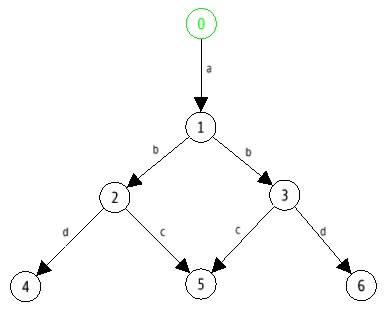
\includegraphics[width=2.5in]{graph1}
% \caption{Graph 1}
% \label{fig:graph1}
% \end{figure}

% \begin{figure}[h!]
% \centering
% 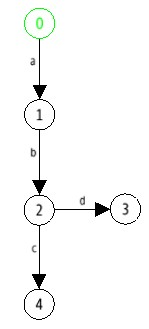
\includegraphics[width=1.0in]{graph2}
% \caption{Graph 2}
% \label{fig:graph2}
% \end{figure}

\begin{figure}[h!]
\centering
\subfigure[Graph 1]{
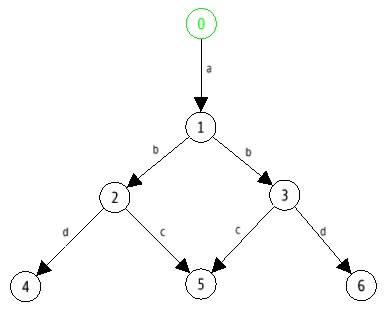
\includegraphics[width=2.3in]{graph1}
\label{fig:graph1}
}
\subfigure[Graph 2]{
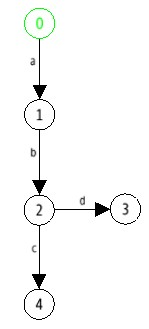
\includegraphics[width=0.9in]{graph2}
\label{fig:graph2}
}
\label{fig:exampleGraphs}
\caption{Example of two labeled graphs}
\end{figure}

\begin{figure}[h!]
\centering
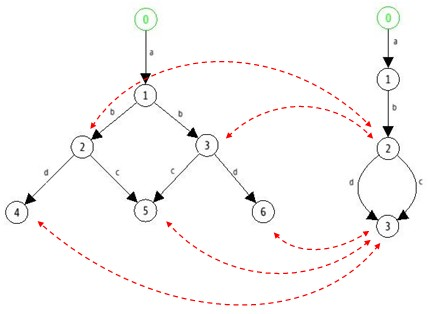
\includegraphics[width=3.0in]{bisimGraph1}
% where an .eps filename suffix will be assumed under latex, 
% and a .pdf suffix will be assumed for pdflatex; or what has been declared
% via \DeclareGraphicsExtensions.
\caption{Minimized Graph 1}
\label{fig:bisimGraph1}
\end{figure}

An illustration of the output of the algorithms for the graphs shown on Fig. 2 and Fig. 3 is given in TABLE I.

\begin{table}[h!]
\begin{tabular}{| l | p{3.2cm}| p{3.2cm} | }
  \hline                       
  Algorithm & Graph 1 & Graph 2 \\ \hline
  Naive & \{(2, 3), (3, 2), (4, 5), 
(5, 4), (4, 6), (6, 4), (5, 6), (6, 5), (0, 0), (1, 1), (2, 2), (3, 3), (4, 4), (5, 5), (6, 6)\} & \{(3, 4), (4, 3), (0, 0), 
(1, 1), (2, 2), (3, 3), (4, 4)\} \\ \hline
  Fernandez & \{\{0\}, \{1\}, \{2\}, \{3\}, \{4, 5, 6\}\} & \{\{0\}, \{1\}, \{2\}, \{3, 4\}\} \\ \hline  
\end{tabular}
\caption{Computing strong bisimularity for Graph 1 and Graph 2}
\label{table1}
\end{table}

The next step uses these results to minimize the graphs. In order to minimize the graphs all bisimular states are merged into
one single state and all mutual incoming and outgoing transitions are merged as well.

The process of reduction of the Graph 1 to its minimal form is given on Fig. 4. As it can be seen from the figure, the states 
2 and 3 are merged into state 2 in the minimal graph, and states 4, 5, and 6 are merged into state 3 in the minimal graph.
\begin{figure}[h!]
\centering
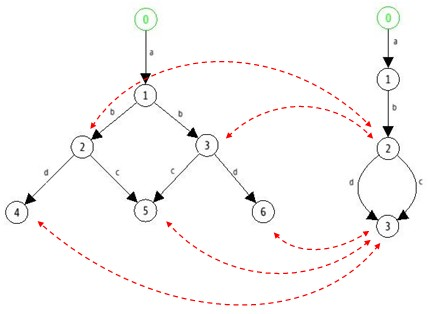
\includegraphics[width=3.0in]{bisimGraph1}
% where an .eps filename suffix will be assumed under latex, 
% and a .pdf suffix will be assumed for pdflatex; or what has been declared
% via \DeclareGraphicsExtensions.
\caption{Minimized Graph 1}
\label{fig:bisimGraph1}
\end{figure}

The process of reduction of the Graph 2 to its minimal form is given on Fig. 5. As before, the states 
3 and 4 are merged into state 3 in the minimal graph.
\begin{figure}[h!]
\centering
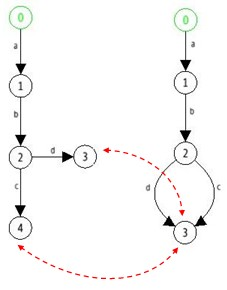
\includegraphics[width=1.8in]{bisimGraph2}
% where an .eps filename suffix will be assumed under latex, 
% and a .pdf suffix will be assumed for pdflatex; or what has been declared
% via \DeclareGraphicsExtensions.
\caption{Minimized Graph 2}
\label{fig:bisimGraph2}
\end{figure}

Having reduced the two labeled graphs into their minimal forms, the last step in the process of checking the equivalence
between the two labeled transition system consists of checking whether the two minimal labeled graphs are isomorphic.

Two graphs g and h are isomorphic if there exists a graph isomorphism between them. According to [ref8], a graph isomorphism 
between two graphs g and h is a bijective function f: Nodes(g) -> Nodes(h) satisfying:
\begin{itemize}
	\item f(initialNode(g)) = g(initialNode(h))
	\item (s, a, t) is an edges in g \Leftrightarrow (f(s), a, f(t)) is an edge in h
\end{itemize}

The two graphs are bisimilar.

The correctness of the implementation was tested with the use of ltsconvert and ltscompare tools of MCRL2, ....[ref6]

\begin{figure}[h!]
\centering
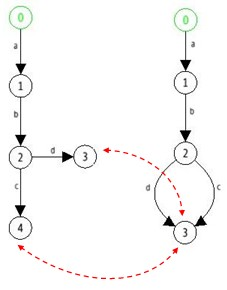
\includegraphics[width=2.0in]{bisimGraph2}
% where an .eps filename suffix will be assumed under latex, 
% and a .pdf suffix will be assumed for pdflatex; or what has been declared
% via \DeclareGraphicsExtensions.
\caption{Minimized Graph 2}
\label{fig:bisimGraph2}
\end{figure}

% [ref1]: Luca Aceto, Anna Ingolfsdottir, Kim G. Larsen and Jiri Srba,
% Reactive Systems - Modeling, Specification and Verification, Cambridge
% University Press, 2007, pages 78-85
% [ref2]: Luca Aceto, Anna Ingolfsdottir, Kim G. Larsen and Jiri Srba,
% Reactive Systems - Modeling, Specification and Verification, Cambridge
% University Press, 2007, pages 85-88
% [ref3]: Aldebaran manual: http://www.inrialpes.fr/vasy/cadp/man/aldebaran.html
% [ref4]: Paige-Tarjan algorithm
% [ref5]: Fernandez
% [ref6}: url za mcrl2
% [ref7]: Model checking
% [ref8]: Handbook of process algebra, page 11,